\chapter{Transport equation problem}
Fluid dynamics and transport phenomena, such as heat and mass transfer, play a vitally important role in human life.\\
Gases and liquids surround us, flow inside our bodies, and have a profound influence on the environment in which we live.\\
 Fluid flows produce winds, rains, floods, and hurricanes.\\ Convection and diffusion are responsible for temperature fluctuations and transport of pollutants in air, water or soil.\\
The ability to understand, predict, and control transport phenomena is essential for many industrial applications,such as aerodynamic shape design, oil recovery from an underground reservoir, or multiphase/multicomponent flows in furnaces, heat exchangers, and chemical reactors.\\
The traditional approach to investigation of a physical process is based on observations, experiments, and measurements. The amount of information that can be obtained in this way is usually very limited and subject to measurement errors.\\
Alternatively, an analytical or computational study can be performed on the basis of a suitable mathematical model. As a rule, such a model consists of several differential and/or algebraic equations which make it possible to predict how the quantities of interest evolve and interact with one another. \cite{tep1}
	\\
\bigskip

The equations and the functionality used in this work, are the same described in the work of a student for the Logic-In-Memory. \\
The transport equation is a partial differential equation that describes the distribution of heat (or variation in temperature) in a given region over time.
\begin{equation}
	\dfrac{\partial}{\partial x} + \dfrac{\partial}{\partial y} = -\dfrac{\partial}{\partial t}
\end{equation}
Temperature values are calculated over a grid and initialized with a gaussian distribution. The points of the grid represent the local indexes (ix, iy) of the matrix that contains the temperature values. The domain is shown in orange in the picture below. Boundaries are represented in white. Data are evolved along Y=X direction, i.e. towards the up-right corner of the coordinate system \cite{lim}.

\begin{figure}[h!]
	\centering
	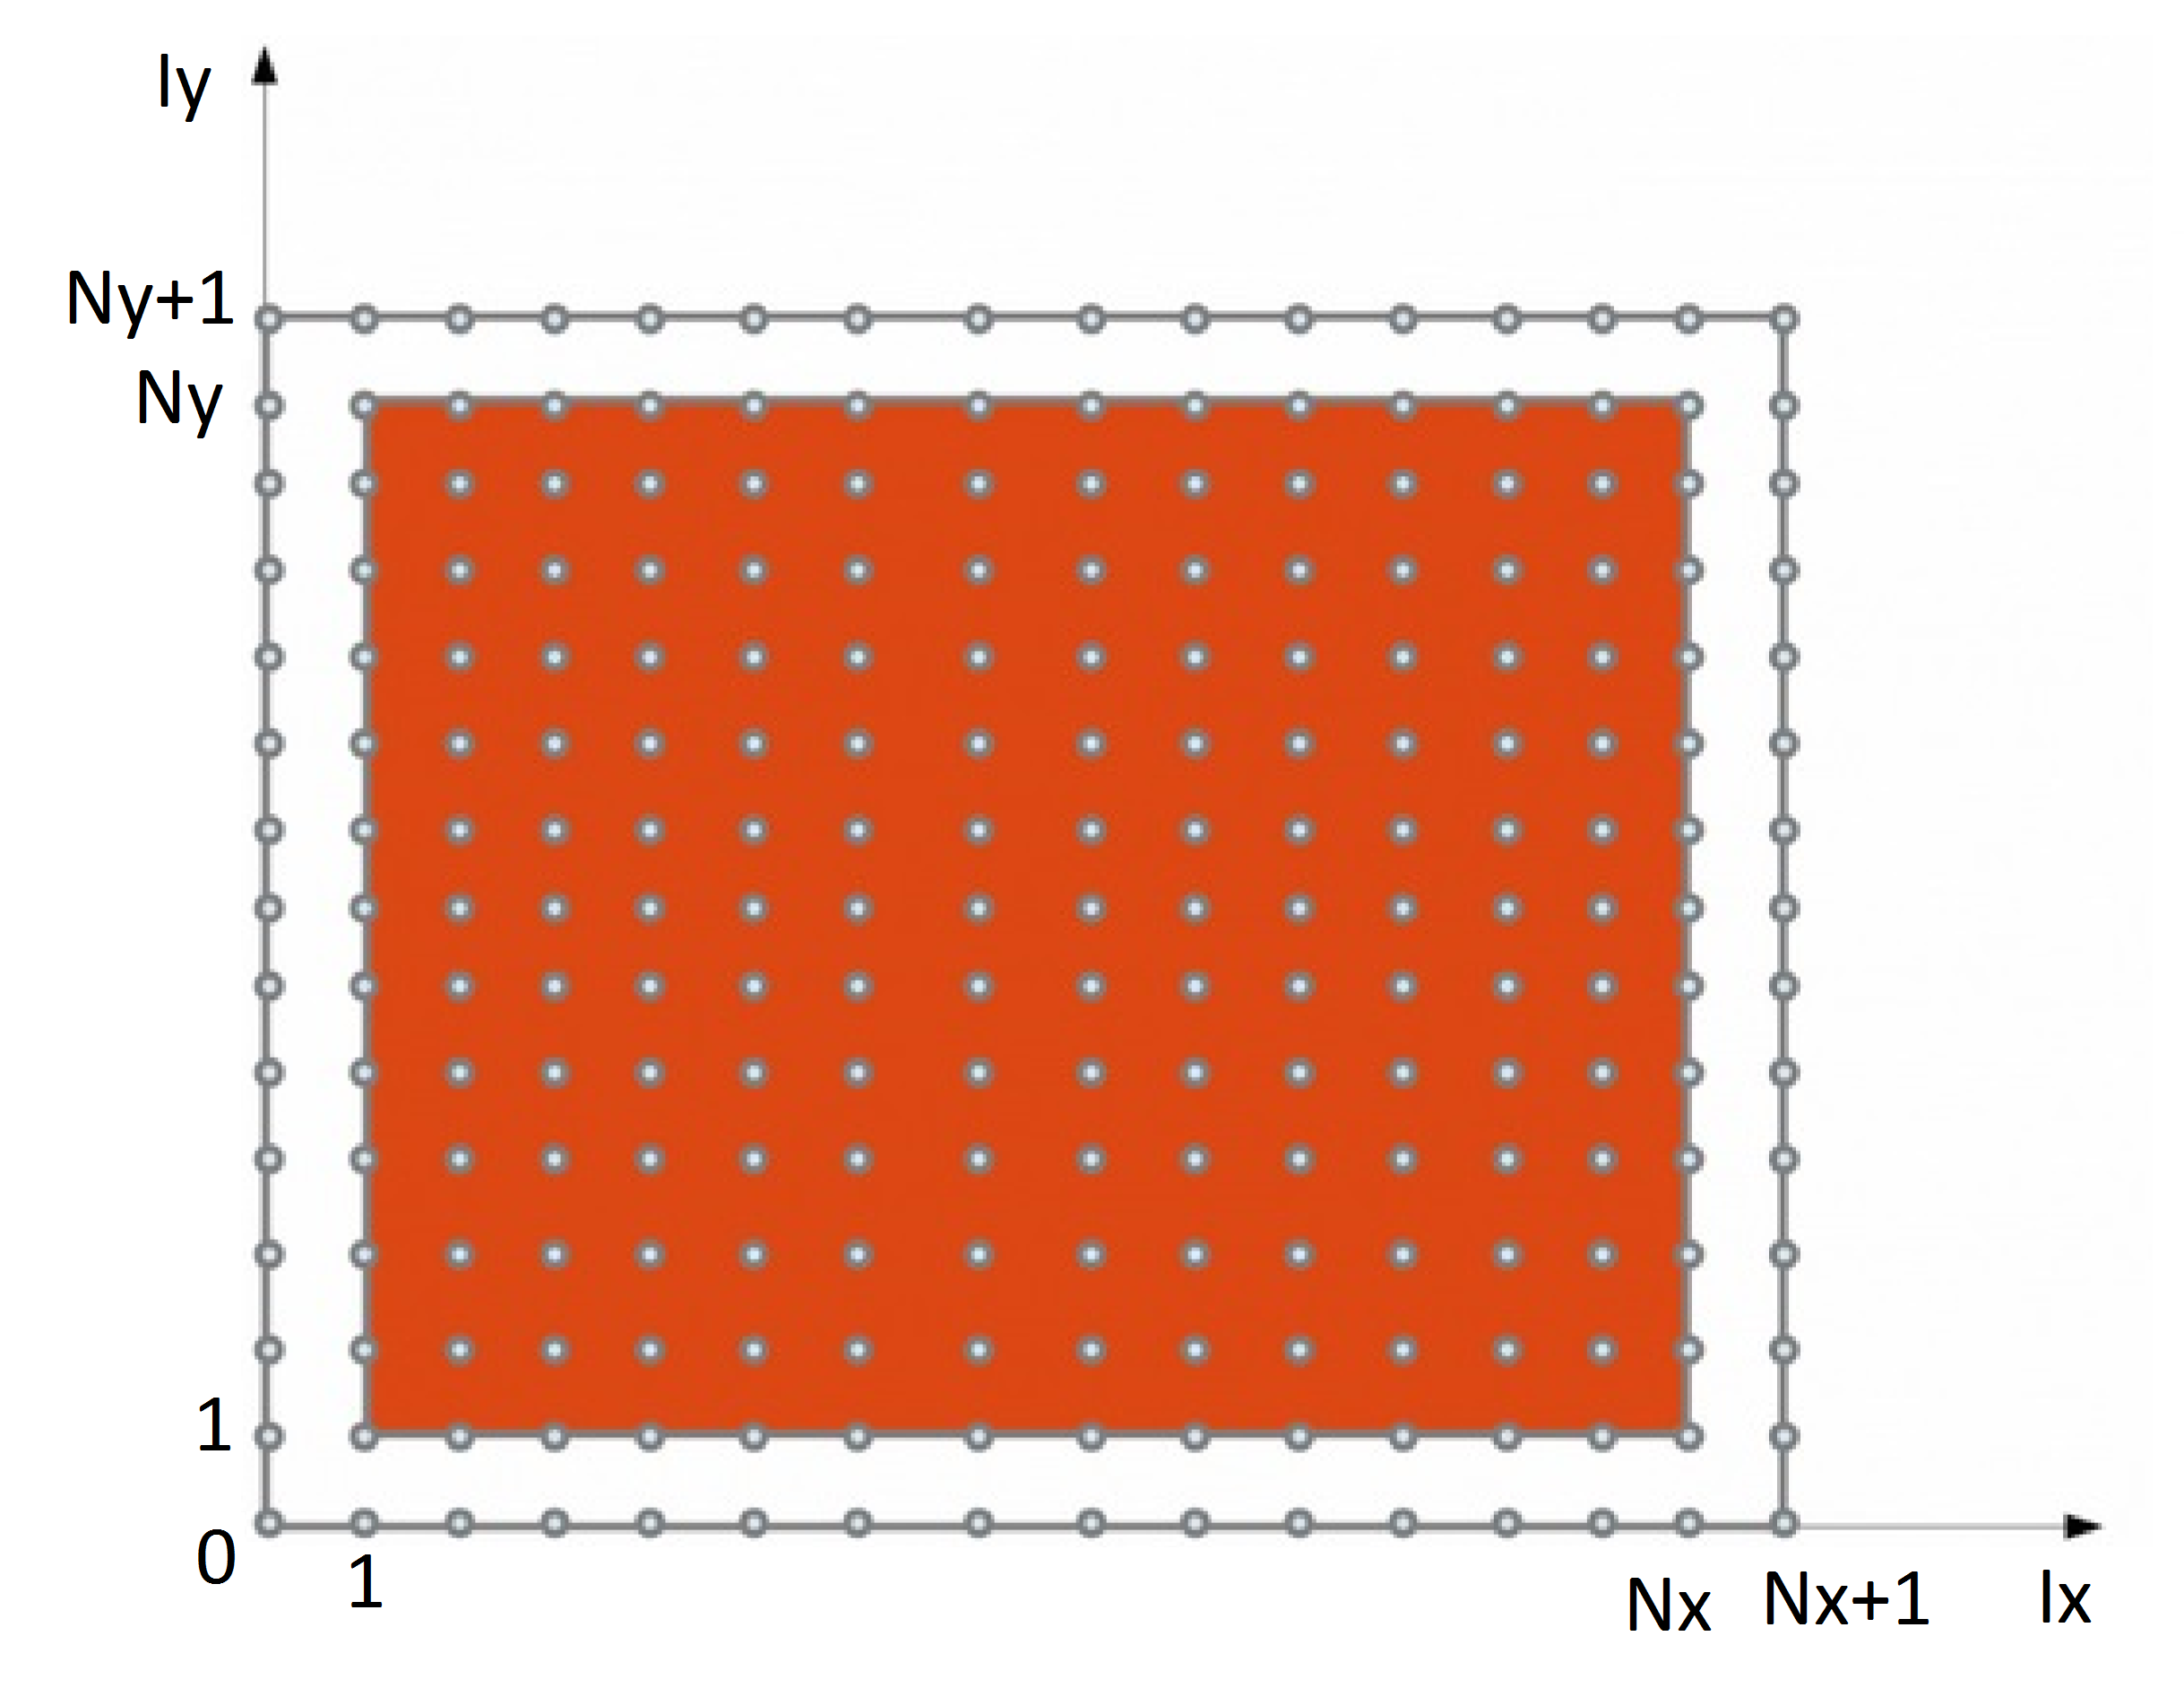
\includegraphics[width=0.8\textwidth]{imm/tep/tep0.png}  
	\caption{Grid for the Transport equation Problem} 
	\label{tep0}
\end{figure}
\bigskip
Each dot of the grid represents a cell. All the cells inside the orange rectangle have to calculate the new value of temperature and the cells at the boundary have to copy the calculated value from the cells at the border of the orange rectangle. Each cell works autonomously performing these calculations: 
\begin{equation}
	temp = t_{0}-\alpha[t(i+1,j)-t(i-1,j)+t(i,j + 1)-t(i,j-1)] 
\end{equation}
As shown below, each cell reads the values of temperature of the adjacent cells to compute the equation illustrated above:
\begin{figure}[h!]
	\centering
	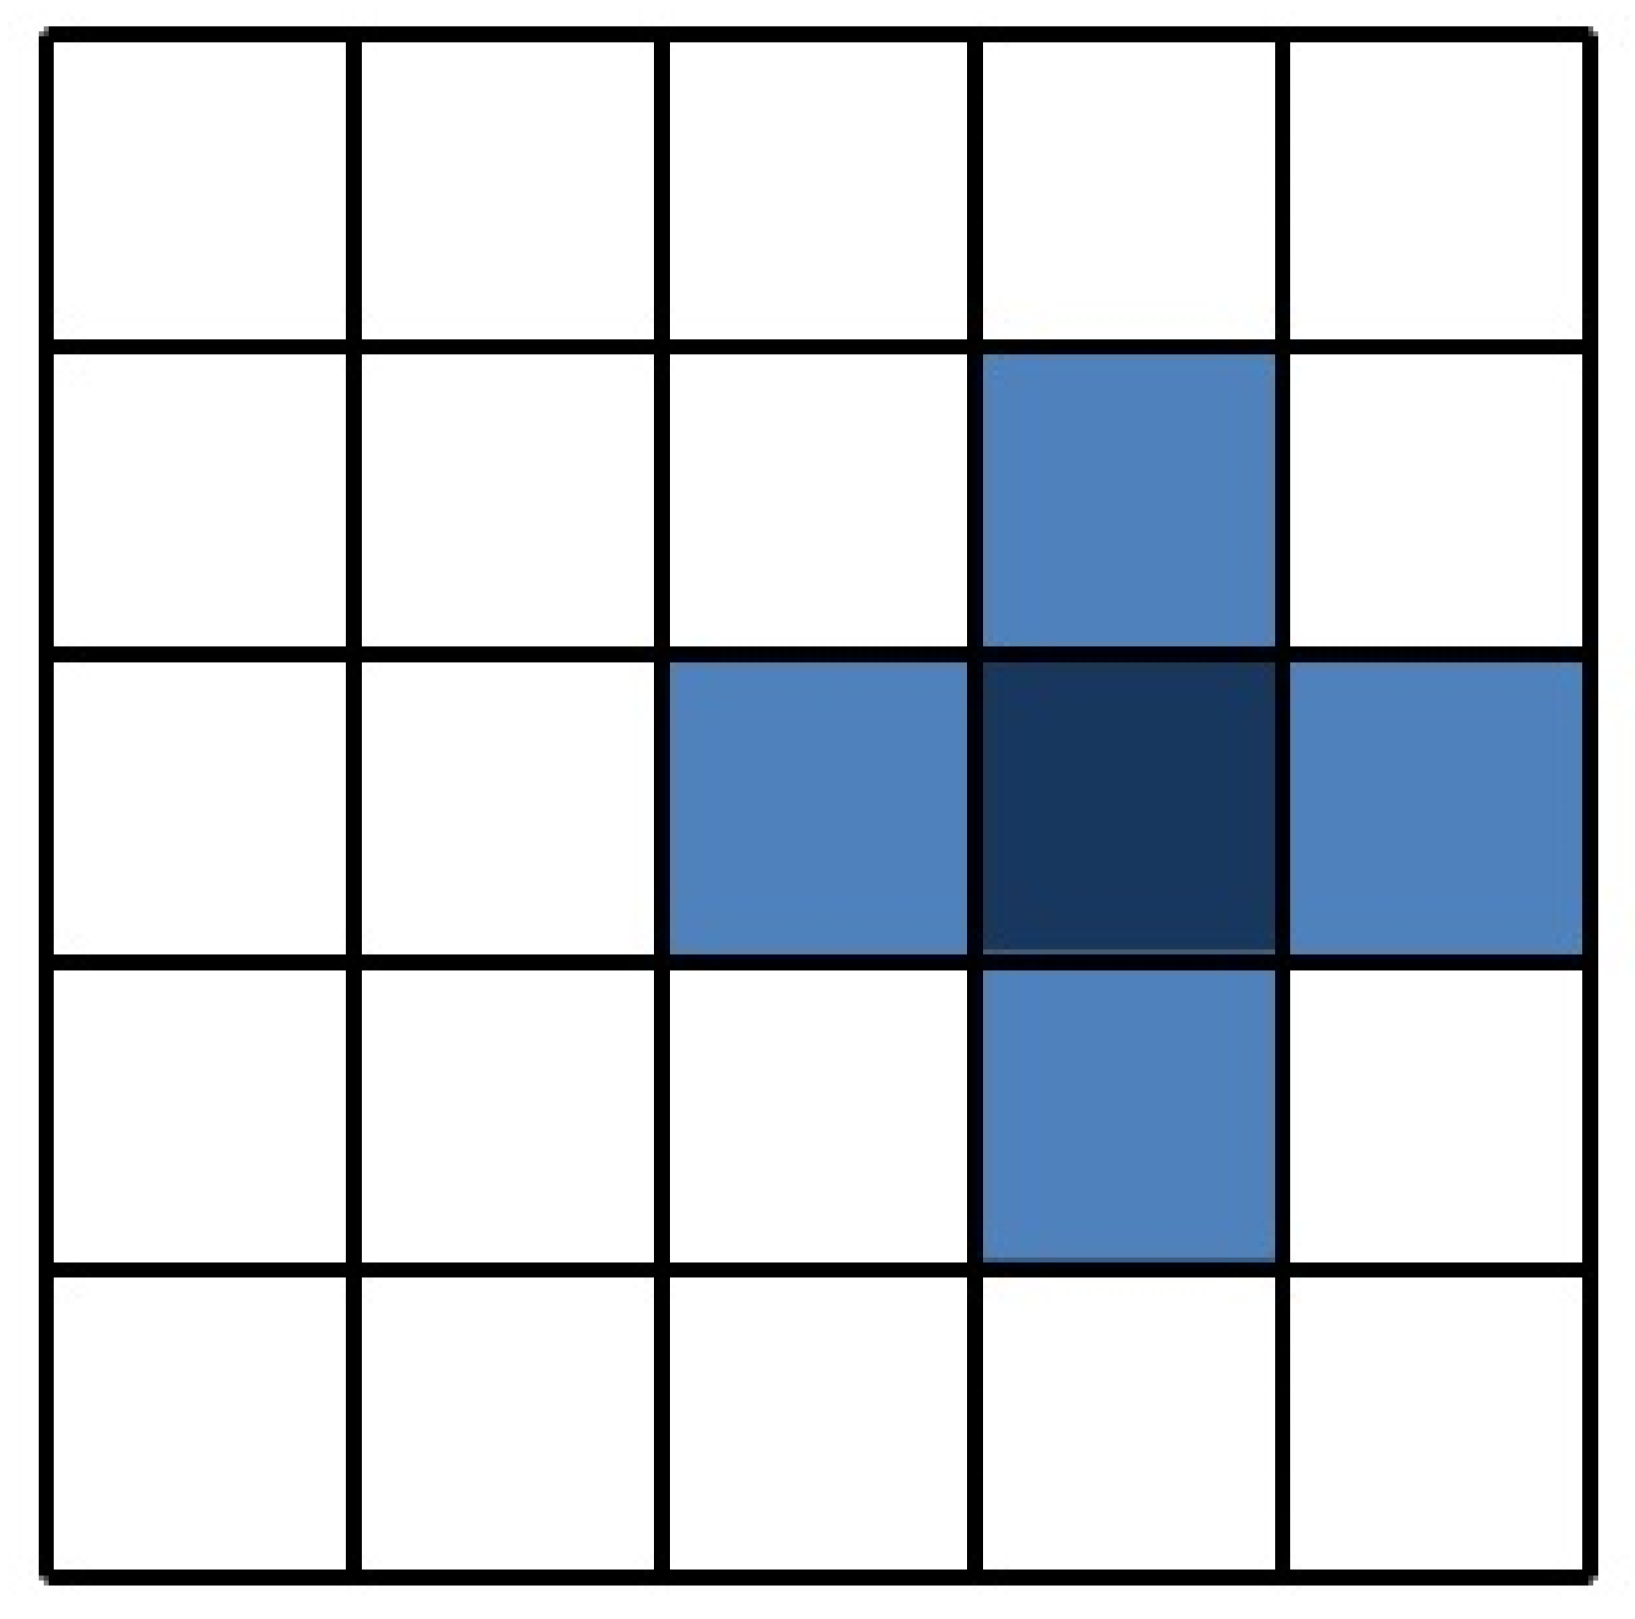
\includegraphics[width=0.5\textwidth]{imm/tep/tep1.png}  
	\caption{Transport Equation Problem for a single cell} 
	\label{tep1}
\end{figure}
After that, the cells near the boundary copy the calculated values to the boundary cells:
\begin{figure}[h!]
	\centering
	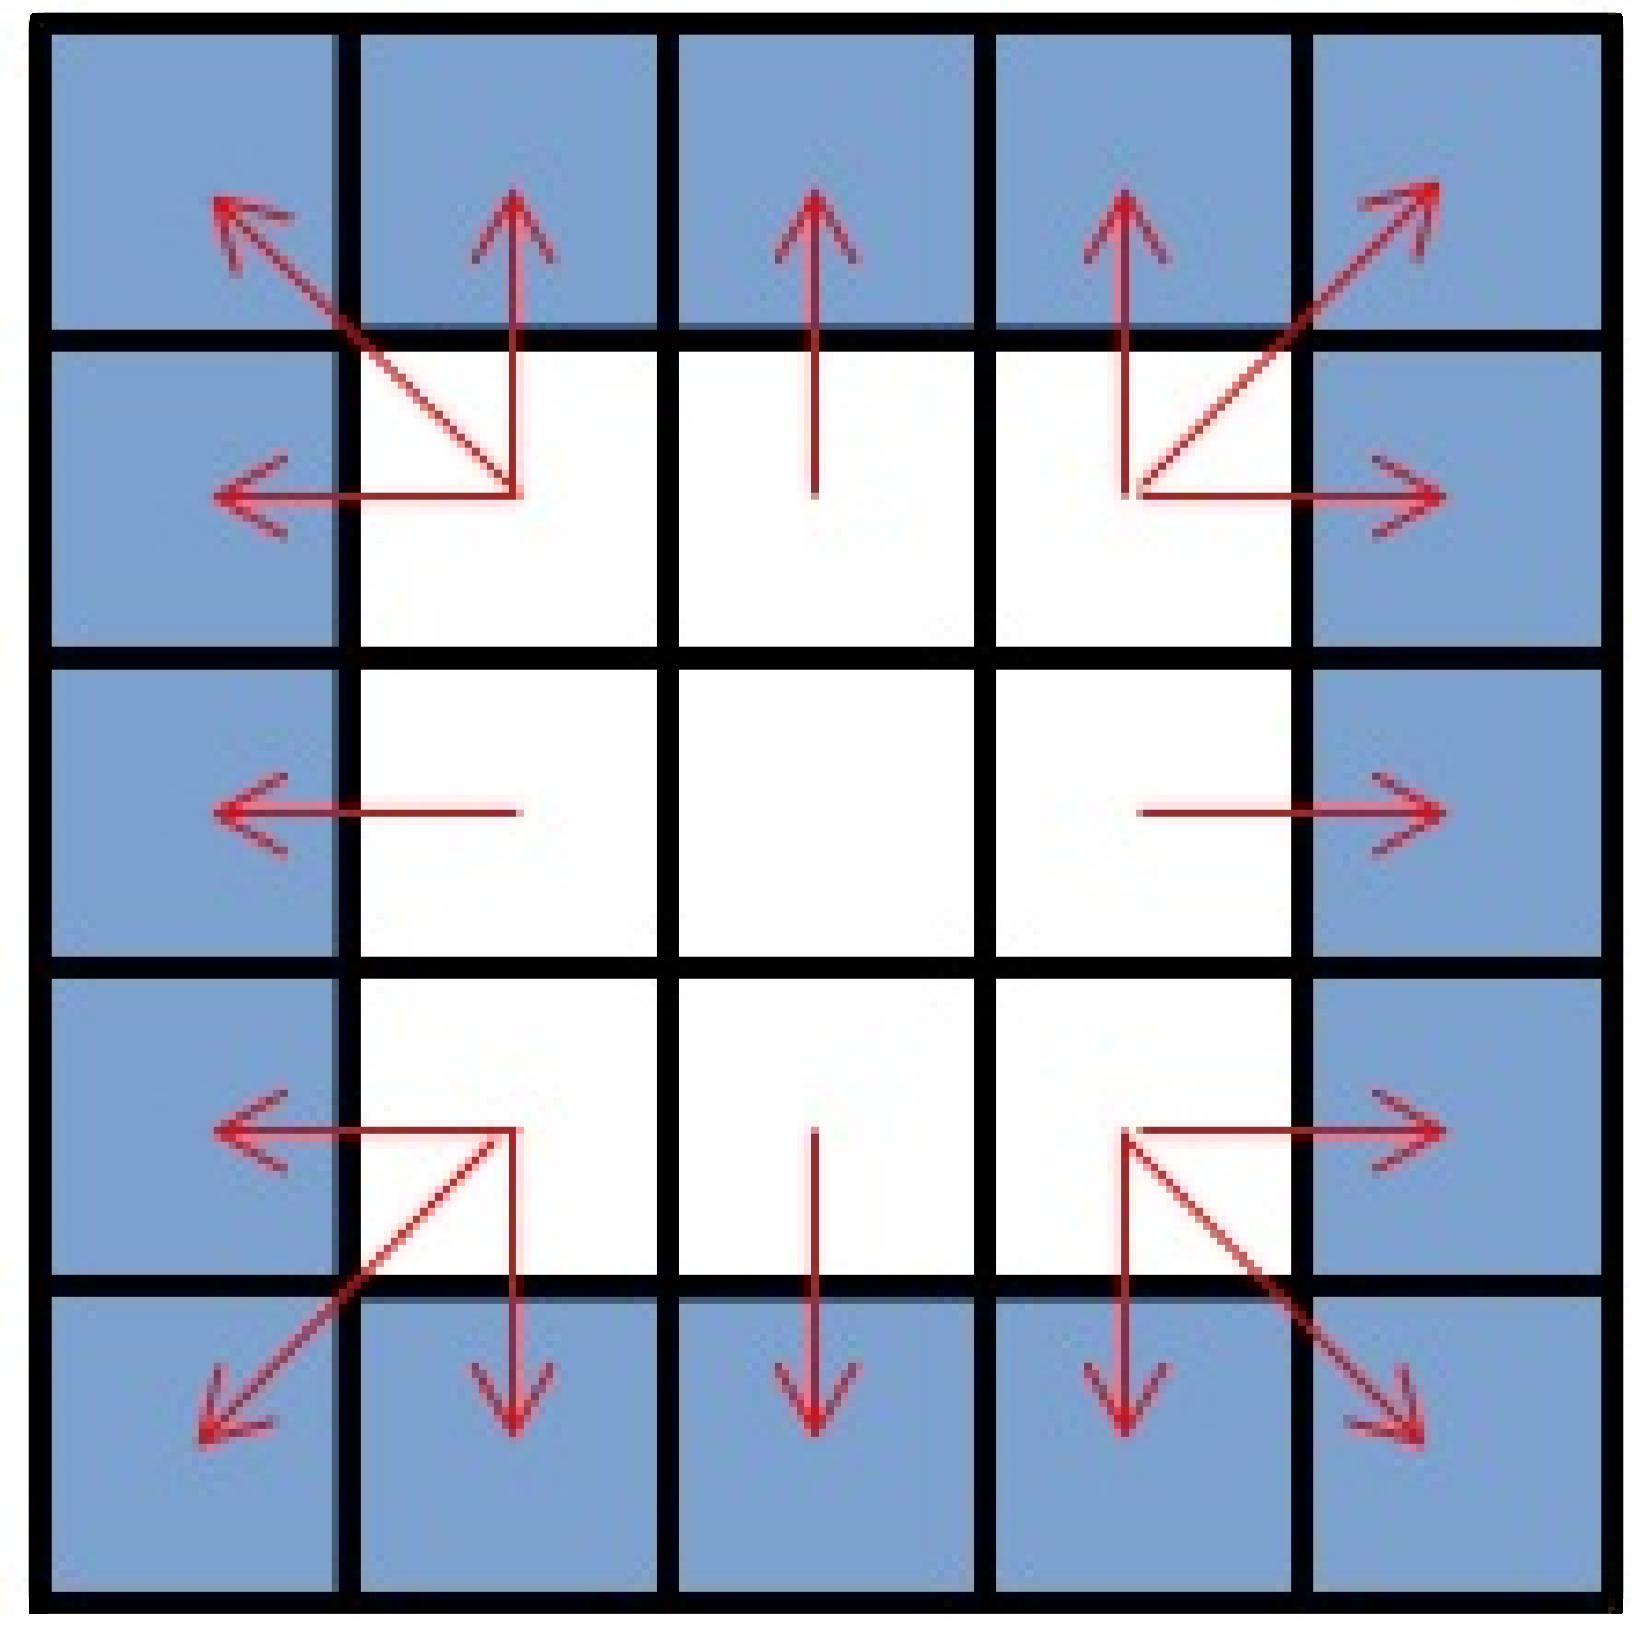
\includegraphics[width=0.5\textwidth]{imm/tep/tep2.png}  
	\caption{Propagarting the values to the boundary} 
	\label{tep2}
\end{figure}

\section{Hardware Implementation}
Since each cell has to compute the same equation, and since there is no data dependencies between them, we can implement a component that compute this result. Let's call it \textit{tep\_unit}.
The \textit{tep\_unit} has as input
\begin{itemize}
\item t0: the value of the interested cell
\item tr: the value of the cell on the right side
\item tup: the value of the cell on the upper side
\item tl: the value of the cell on the left side
\item tdn: the value of the cell on the lower side
\item alpha : the value of theconstant
\end{itemize}
with these values, it is possible to  calculate the final value.\\
The equation above can be rewritten as :
\begin{equation} \label{tep_eq2}
temp = t_{0}+\alpha{[t(i-1,j)+t(i,j-1)]-[t(i+1,j)+t(i,j + 1)]}
\end{equation}
For the cell on the border or on the angle of the matrix, we will compute the equation as if there were some zero cells in the neighborhood.
In fig. \ref{tep_unit} we can see the DFG.
\begin{figure}[h!]
	\centering
	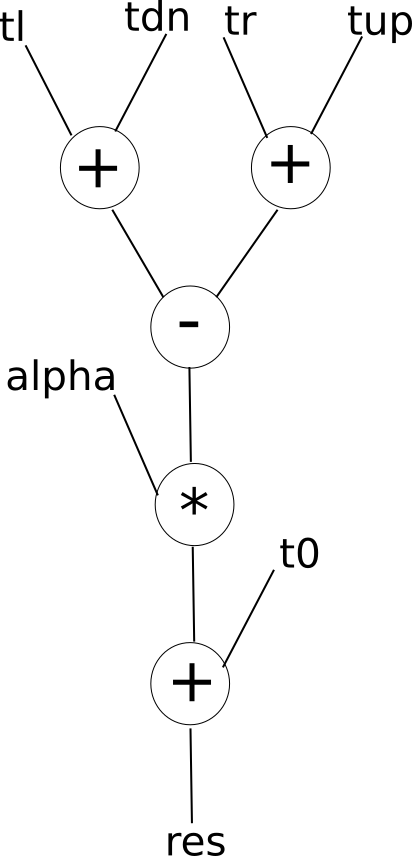
\includegraphics[width=0.4\textwidth]{imm/tep/tep_unit0.png}  
	\caption{Tep\_unit DFG} 
	\label{tep_unit}
\end{figure}

\clearpage
\newpage
\section{Simulation}
The simulation shown in this work has a 4x4 matrix  (fig. \ref{fig:tep_sim}, highlighted in yellow)
\begin{center}
	$\begin{bmatrix}
	1 & 2& 3&4\\
	3&4&2&8\\
	5&6&1&18\\
	7&8&0&22
	\end{bmatrix}$
\end{center}
\begin{figure}[h!]
	\centering
	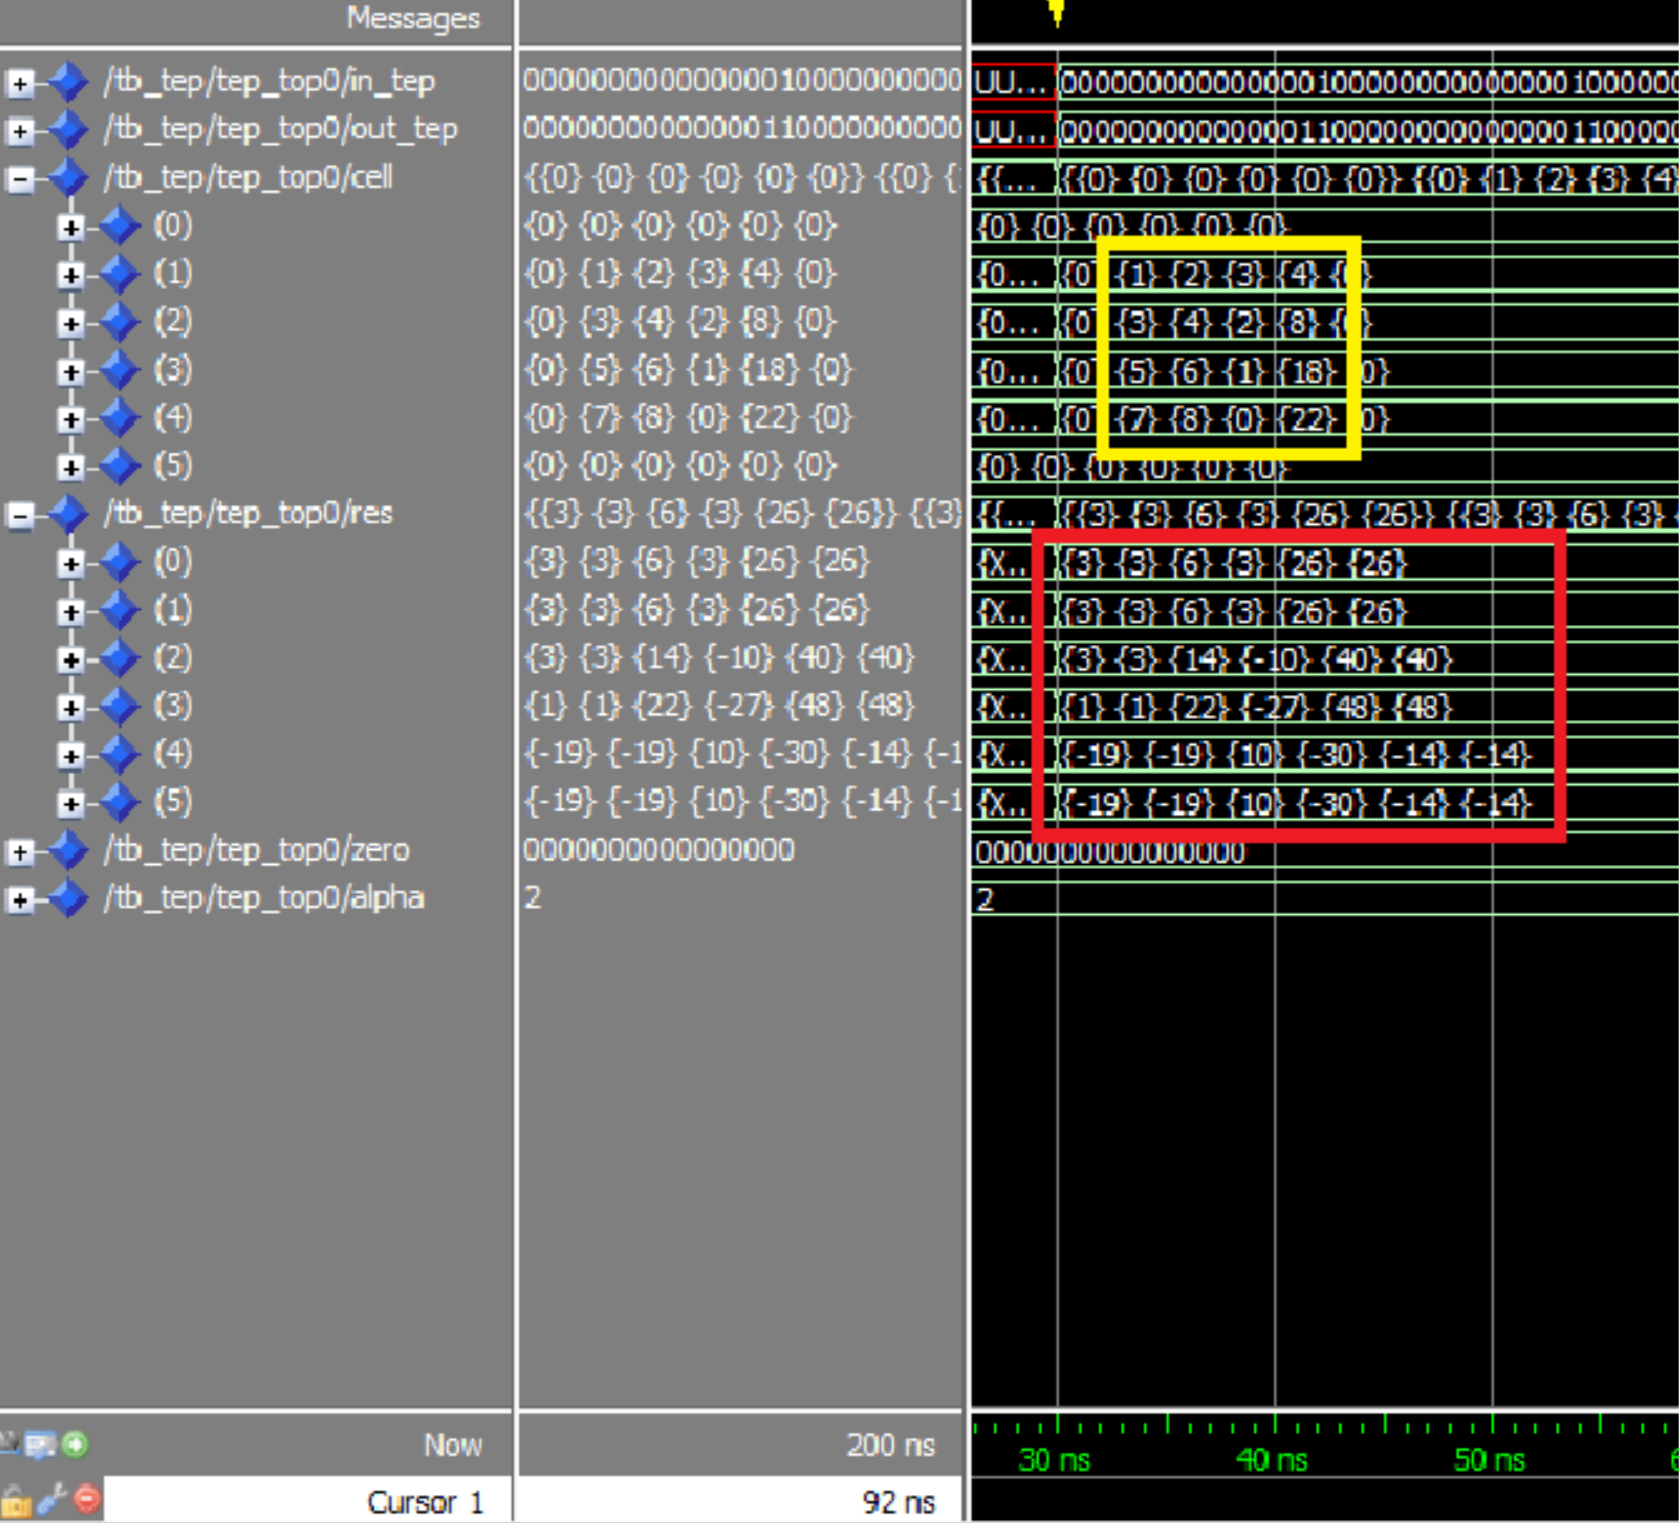
\includegraphics[width=\textwidth]{imm/tep/wave_t.png}  
	\caption{Transport Equation Problem's simulation} 
	\label{fig:tep_sim}
\end{figure}
\bigskip
If we compute the equation \ref{tep_eq2} for each element we will get 
\begin{center}
	$\begin{bmatrix}
	3 & 6& 3&26\\
	3&14&-10&40\\
	1&22&-27&48\\
	-19&10&-30&-14
	\end{bmatrix}$
\end{center}
\bigskip
Now we have to propagate the values on the border to the boundary, thus having
\begin{center}
	$\begin{bmatrix}
	3&3 & 6& 3&26&26\\
	3&3 & 6& 3&26&26\\
	3&3&14&-10&40&40\\
	1&1&22&-27&48&48\\
	19&-19&10&-30&-14&-14\\
	19&-19&10&-30&-14&-14
	\end{bmatrix}$
\end{center}
\bigskip
\section{Comparison with LIM's architecture}
I take the results of the LIM's architecture. 
The pseudocode for the LIM architecture is the following:
\begin{enumerate}
 \item Each cell reads its own value; 
 \item Reads N-W-S-E cells data (4 different values);
 \item Computes sums/subtractions and a multiplication; 
 \item Boundary cells just copy their neighbours' values;
 \item Writes the final result in its own memory;
\end{enumerate}
As already said, the main advantage of the LIM architecture is the parallelism: the presence of many cells that can work autonomously greatly increases the speed of the computation of algorithms that can be executed in parallel.\\
In particular, the duration of the algorithms doesn't depend on the number of cells composing the grid.
The total duration for the computation is equal to:
\begin{itemize}
\item $ N $ clock cycles to write the data;
 \item $ 16 \cdot i  $clock cycles to compute the algorithm;
 \item $ 2N+1 $ clock cycles to read the data through a remote read.\\
\end{itemize}
Therefore,
\begin{center}
	$ t =  N + 16\cdot i +2N +1=3N + 16\cdot i +1  $
\end{center}
   \begin{center}
   	\begin{tabular}{ | p{1.8cm} | >{\centering\arraybackslash}p{6cm} | >{\centering\arraybackslash}p{6cm} | }
   		\hline
   		\label{table:tep_tab} & LIM & This work \\
   		\hline
   		Area & $ N^{2}$  cells   & $3N^{2}
   		$  adders, $N^{2}$ substractors, multipliers \\
   		\hline
   		Time & $3N + 16\cdot i +1 $&
   		
   		(time for 3 additions) + time for a single multiplication 
   		\\
   		\hline
   		
   	\end{tabular}
   \end{center}
   \clearpage
   \newpage
   \section{Characteristics of Transport Equation Problem}
   \vspace{10pt}
   {\large \textbf{PROCESSING ELEMENTS}}\vspace{10pt}\\
   \begin{tabular}{ p{0.2cm} p{14.5cm}}
   	
   	&\textbf{1- Which kind of Processing element?}\\
   	&	Adder, multiplier, substractors\vspace{7pt}\\
   	&	\textbf{2- Functionality}\\
   	&	Addition, multiplications, substractions.\vspace{7pt}\\
   	&	\textbf{3- Complexity}\\
   	&	\begin{tabular}{ p{0.2cm} p{1.2cm}  p{13cm}}
   		
   		& Area: &$ 3N^2 $ adders\\
   		& & $N^2$ substractors\\
   		& & $N^2$ multipliers\\
   		& Time: &Time for one  one multiplication and  $3 $ additions \vspace{3pt}\\
   		
   		
   	\end{tabular}\vspace{7pt}\\
   	&	\textbf{4- Parallelism}\\
   	&	Each cell can evaluate their Transport Equation Problem output\vspace{7pt}\\
   	&	\textbf{5-Reconfigurability}\\
   	&	No\vspace{7pt}\\
   	&	\textbf{6- Programmability}\\
   	&	No\vspace{7pt}\\
   	&	\textbf{7- Need a dedicated memory?}\\
   	&	No\vspace{7pt}\\
   	&\textbf{8- Relationship with I/O}\\
   	&	INPUT: values of the cells in the matrix\\
   	&	OUTPUT: result of the Transport Equation Problem. algorithm\end{tabular}\vspace{74pt}\\
   \newpage{\large \textbf{\qquad }}\vspace{10pt}\\
   {\large \textbf{MEMORY ELEMENTS}}\vspace{10pt}\\\begin{tabular}{ p{0.2cm} p{14.5cm}}
   	&\textbf{1- Need a clever memory LIM?}\\
   	&	No, but can be implemented\vspace{7pt}\\
   	&\textbf{2- Is there a data search algorithm?}\\
   	&	No\vspace{7pt}\\
   	&\textbf{	3-Interface mechanism with other PE or memories}\\
   	&	Communication required between local elements\vspace{7pt}\\
   	&	\textbf{4- Access mechanism}\\
   	&	(No memory for this implementation)\vspace{7pt}\\
   	&	\textbf{5- Hierarchization} \\
   	&	(No memory for this implementation)\vspace{7pt}\\
   	&\textbf{	6- Cache coherency} \\
   	&	(No memory for this implementation)\vspace{7pt}\\
   	&\textbf{	7- Is it a a transactional memory?}\\
   	&	(No memory for this implementation)\vspace{7pt}\\
   	&\textbf{	8- Are there virtualization (paging) mechanisms?}\\
   	&	(No memory for this implementation)\end{tabular}\vspace{14pt}\\
   \vspace{10pt}\\
   {\large\textbf{ENCODING INFORMATION}}\vspace{10pt}\\
   \begin{tabular}{ p{0.2cm} p{14.5cm}}
   	&\textbf{1-Which encoding is used?}\\
   	&Binary encoding
   \end{tabular}
   \newpage{\large\textbf{ }}\vspace{10pt}\\
   {\large\textbf{CONNECTIONS}}\vspace{10pt}\\\begin{tabular}{ p{0.2cm} p{14.5cm}}
   	&\textbf{1-Packet Exchange Protocol}\\
   	&Directly\vspace{7pt}\\
   	&\textbf{2-Timing (asynchronou/synchronous)}\\
   	&Synchronous\vspace{7pt}\\
   	&\textbf{3-Are there multiple instances? }\\
   	&Yes\vspace{7pt}\\
   	&\textbf{4-Heterogeneity (Local/Distant I/O Connections)}\\
   	&Heterogeneous. Each cell exchanges data with local cells (No connections between distant cells)\vspace{7pt}\\
   	&\textbf{5-Are there any buffers?}\\
   	&No.
   \end{tabular}\vspace{14pt}\\
   